%\section{Epipolar Geometrie}
%\label{sec:epipolar} 
%
%Kurze zusammenfassung bis hier her..
%%\textcolor{red}{Epipolar geometry is central to stereovision. On the one hand, knowing
%%	it enables to strongly constrain the problem of matching two images.
%%	On the other hand, it can be estimated from matches and then allows
%%	for motion estimation, self-calibration, and triangulation of 3D points
%%	or other geometric primitives.\cite{CamerModels.}}
%
%Die Epipolargeometrie beschreibt ähnlich der Homographie eine Beziehung der projektiven Geometrie zwischen zwei Bildern\cite{HZ}. Sie dient insbesondere zur Korrespondenzanalyse von Punkten aus Bildern und zur Gewinnung von 3D-Informationen die abgebildete Szene. Im Gegensatz zur Homographie ist die Epipolargeometrie unabhängig vom Szenenaufbau, sondern hängt nur von den intrinsischen Parametern der Kamera, sowie deren relative Position zueinander ab.\cite{HZ}. Ohne Kenntnis der Kamerapositionen, kann mit Hilfe der Epipolargeometrie überprüft werden, ob eine Korrespondenz zwischen den Bildpunkten zweier Bilder besteht. Unter korrespondierenden Punkten versteht man Bildpunkte auf zwei Bildern, die Abbilder des selben Objektpunktes im 3D-Raum sind. Ein Beispiel für korrespondierende Punkte wären die Punkte Bildpunkte $m_\tau$ und $m_\tau'$. Diese entstanden aus der Projektion von $M_\delta$ auf zwei Bildebenen mit $m_\tau = PM_\delta$ und $m'_{\tau'} = P'M_\delta$. Die Verbindungsvektoren zwischen den Projektionszentren $C$ und $C'$ mit dem 3D-Objektpunkt $M_\delta$ und die Basislinie, welche die Projektionszentren verbidnet, bilden die Epipolarebene. Auf Abbildung \ref{fig:Epipolargeometry} ist sie als Dreieck zwischen den Punkten zu sehen. Die Epipolargeometrie beschreibt in die Beziehung zwischen den durch Schnitt der Bildebenen und der Epipolarebene entstehenden Schnittgeraden. Für jeden Objektpunkt im Raum, entsteht eine neue solche Ebene, die alle die Basislinie als Drehachse besitzen\cite{HZ}. Dementsprechend entstehen pro neuen Opbjektpunkt im Raum auch jeweils zwei Schnittgeraden. Die Schnittgeraden werden als Epipolarlinien $l$ und $l'$ bezeichnet. $l'$ wird als die zu zum Bildpunkt $m_\tau$ korrespondierende Epipolarlinie bezeichnet und $l$ die zum Bildpunkt $m'_{\tau'}$ korrespondierende Epipolarlinie.  Die Epipolarlinien eines Bildes verlaufen alle durch einen Epipol $e$ oder $e'$ und den abgebildeten Bildpunkten und bilden somit,auf den jeweiligen Bildebenen, ein Bündel aus Epipolarlinien. Epipol $e$ ist die Abbildung von $C'$ auf der Bildebene $I$ von $C$ und Epipol $e'$ ist die Abbildung von $C$ auf Bildebene $I'$ von $C'$. Die Schnittpunkte der Basislinie mit den Bildebenen ergeben die jeweiligen Epipole. Ist eine der Bildebenen parallel zur Basislinie ausgerichtet, so kommt es zu keinem Schnittpunkt der Basislinie mit der parallelen Bildebene und der Epipol befindet sich somit im unendlichen\cite{HZ,ZZGXr}.
%
%\begin{minipage}{\linewidth}
%	\centering
%	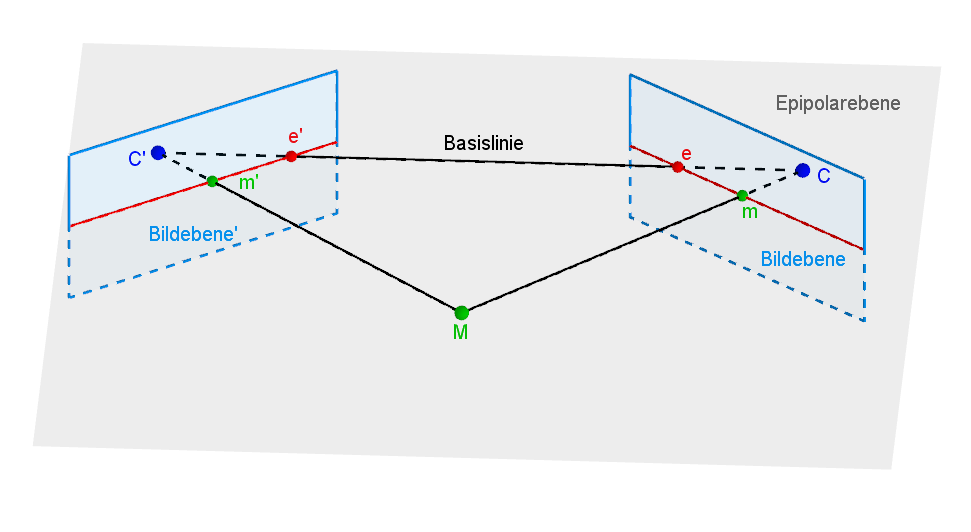
\includegraphics[width=.8\linewidth]{images/EpipolarGeoemtrieGrafik.png}
%	\captionof{figure}{$C$ und $C'$ sind die Projektionszentren zweier Kameras. Beide Kameras besitzen jeweils eine Bildebene. Die Basislinien verbindet die Projektionszentren der Kameras. Der Punkt an welchem die Basislinie die Bildebenen schneidet, wird als Epipol bezeichnet. Durch den Epipol verlaufen alle Epipolarlinien des Bildes. $M$ ist der Objektpunkt im 3D-Raum und $m_1$ und $m_2$ sind die jeweiligen Abbildungen dieses Punktes auf den Bildebenen. Die Verbindungsvektoren zwischen $C, C'$ und $M$ bilden die sogenannte Epipolarebene\cite{Elements,HZ,ZZGXr}.}  
%	\label{fig:Epipolargeometry}
%\end{minipage}\\ \\
%
%Ein Objektpunkt $M_\delta$ wird auf die Bildebenen $I$ und $I'$ der beiden Kameras $C$ und $C'$ projiziert. Es entstehen die zueinander korrespondierenden Bildpunkte $m_\tau$ und $m'_{\tau'}$. Die durch die Bildpunkte $m_\tau$ und $m'_{\tau}$ und den entsprechenden Epipolen $e$ und $e'$ verlaufenden Epipolarlinien, sind zueinander korrespondierende Epipolarlinien. Die zum Punkt $m_\tau$ korrespondierende Epipolarlinie $l'$ beinhaltet alle zu $m_\tau$ möglichen korrespondierenden Punkte, darunter eben auch der eindeutig korrespondierende Punkt $m'_{\tau'}$. Die Epipolargeometrie beschreibt weiterhin eine Beziehung zwischen einem Bildpunkt $m$ und dessen korrespondierender Epipolarlinie $l'$. Diese Beziehung ist der sogenannte ist der sogenannte \textit{Epipolar-Constraint}\cite{HZ,Zhang2014,ZZGXr}. Abbildung \ref{fig:Epipolarconstraint} veranschaulicht die soeben genannte Beziehung eines Bildpunktes zu seiner korrespondierenden Epipolarlinie noch mal grafisch. Der \textit{Epipolar-Constraint} sagt aus, dass wenn ein 3D-Bildpunkt $M_\delta$ sich entlang seiner Verbindungslinie $\overline{CM_\delta}$ auf die Bildebene $I$ zu bewegt, so ändert sich die Position des Bildpunktes $m_\tau$ auf $I$ nicht,während der korrespondierende Punkt $m'_{\tau'}$ sich entlang seiner Epipolarlinie bewegt. In Abbildung \ref{fig:Epipolarconstraint} ist $m_\tau$ mit $m_{\tau,i}$ bezeichnet. Ist also nur Bildpunkt $m_\tau$ bekannt, so können alle Punkte auf dessen korrespondierender Epipolarlinie $l'$ mögliche korrespondierende Punkte zu $m_\tau$ sein. Der \textit{Epipolar-Contraint} kann durch $3 \times 3$-Matrizen ausgedrückt werden. Bei diesen Matrizen handelt es sich entweder um die Fundamentalmatrix $F$ oder die essentielle Matrix $E$\cite{HZ,ZZGXr,Elements,CamerModels.,Zhang2014}. Deren Herleitung und Beziehung, zu den korrespondierenden Bildpunkten, im weiteren Verlauf noch aufgezeigt wird. Der \textit{Epipolar-Contraint} gilt dann als erfüllt, wenn gilt, dass:
%
%
%
%\begin{gather}
%	m'^T_{\tau'} \cdot F \cdot m_\tau = 0\\
%	\bar{m}'^T_{\tau'} \cdot E \cdot \bar{m}_{\tau} = 0
%\end{gather}
%
%ergeben. Sind die Gleichungen erfüllt, dann sagt der\textit{Epipolar-Constraint} aus, das Bildpunkt  $m'_{\tau'}$ auf der zu $m_\tau$ korrespondierenden Epipolarlinie $l'$ liegt und somit ein möglicher korrespondierender Punkt zu $m_\tau$\cite{HZ,Zhang2014,Elements,ZZGXr}. Ist der \textit{Epipolar-Constraint} erfüllt, so wird gleichzeitig der Suchaufwand nach weiteren Korrespondenzen reduziert, da somit nur noch eine eindimensionale Suche, entlang der Epipolarlinie, anstatt einer zweidimensionalen durchgeführt werden muss. Dieser neue \textit{Contraint} wird auch als \textit{Coplanarity-Constraint} oder Koplanaritätsbeschränkung bezeichnet. Er sagt aus, dass die Projektionszentren der Kameras und die korrespondierenden Bildpunkte auf ein und der selben Epipolarebene liegen müssen \cite{Zhang2014}.
%
%
%\begin{minipage}{\linewidth}
%	\centering
%	\includegraphics[width=1.\linewidth]{images/EpipolarLinien.png}
%	\captionof{figure}{Die Objektpunkte $M_1, M_2$ und $M_3$ werden in $I'$ als $m'_1, m'_2$ und $m'_3$ abgebildet, während sie in $I$ immer den selben Bildpunkt $m_1$ ergeben.}  
%	\label{fig:Epipolarconstraint}
%\end{minipage}\\ \\
%
%Die essentielle Matrix und die Fundamentalmatrix unterscheiden sich darin, ob die intrinsischen Kameraparameter bekannt sind oder nicht. Die Fundamentalmatrix kommt dann zum Einsatz, wenn nur die Bildpunkte $m_\tau$ und $m'_{\tau'}$ bekannt sind, die Kameramatrizen $K$ und $K'$ und die Translationsmatrizen $R$ und $R'$ jedoch unbekannt sind. Man spricht hier von einem unkalibrierten Fall\cite{HZ,ZZGXr,Ferid}. Sind die intrinsischen Kameraparameter bekannt, so wird die Fundamentalmatrix $F$ zur essentiellen Matrix und man spricht von einem kalibrierten Fall$E$\cite{HZ,Elements}. Das Wissen über die Aussagen dieser \textit{Constraints} ist vor allem dann von Nutzen, wenn es darum geht aus einer Stereoskopischen Aufnahme anhand von korrespondierenden Bildpunkten die 3D-Szene zu rekonstruieren. Die korrespondierenden Punkte müssen zu Beginn der Stereobildanlayse erst einmal auf den Bilder ausfindig gemacht werden. Hierfür gibt es unterschiedliche Algorithmen, die in der \nameref{sec:einleitung} bereits erwähnt wurden. Wird einer dieser Algorithmen auf die Bilder angewandt, kann mit Hilfe des \textit{Epipolar-Constraints} deren Exaktheit der zueinander korrespondierenden Punkte überprüft werden\cite{Elements,ZZGXr,HZ}. 

